\documentclass[12pt,twoside]{article}
\usepackage{amsmath, amssymb}
\usepackage{amsmath}
\usepackage{fancyhdr,parskip}
\usepackage[active]{srcltx}
\usepackage{amssymb}
\usepackage{amscd}
\usepackage{makeidx}
\usepackage{amsthm}
\usepackage{algorithm}
\usepackage{algpseudocode}
\usepackage{fancyhdr}
\usepackage{graphics}
\usepackage{amsmath, amssymb}
\usepackage{amsmath}
\usepackage[active]{srcltx}
\usepackage{amssymb}
\usepackage{amscd}
\usepackage{makeidx}
\usepackage[dvips]{graphicx}
\usepackage{longtable}
\usepackage{tabularx}
\usepackage[table,xcdraw]{xcolor}
\usepackage{color}
\usepackage[hidelinks]{hyperref}
\usepackage[backend=biber,style=apa]{biblatex}
\usepackage{longtable}
\usepackage{tabularx}
\usepackage[table,xcdraw]{xcolor}
\usepackage{color}
\usepackage[hidelinks]{hyperref}
\usepackage{multirow}
\usepackage{algorithm}
\usepackage{algpseudocode}
\usepackage{fancyhdr,graphicx,amsmath,amssymb}
\usepackage{tikz}
\renewcommand{\algorithmicrequire}{\textbf{Input:}}
\renewcommand{\algorithmicensure}{\textbf{Output:}}
\renewcommand{\tablename}{Tabla}
\renewcommand{\figurename}{Figura}
\renewcommand{\baselinestretch}{1}
\setcounter{page}{1}
\setlength{\textheight}{21.6cm}
\setlength{\textwidth}{14cm}
\setlength{\oddsidemargin}{1cm}
\setlength{\evensidemargin}{1cm}
\pagestyle{myheadings}
\thispagestyle{empty}
\markboth{\small{Pr\'actica 4. Luis Francisco Renteria Cedillo, Denzel Omar Vazquez Perez.}}{\small{.}}
\date{}
\begin{document}
    \begin{figure}[h]
    \vspace{-3cm} \hspace{-2cm} \setlength{\unitlength}{1mm}
    \begin{picture}(15,25)(-10,0)
    
\includegraphics[width=16.5cm,height=2.8cm]{imagenes/titulo.png}
    \end{picture}
    \end{figure}
    \vspace{0cm}
    \centerline{\bf An\'alisis de Algoritmos, Sem: 2022-2, 3CV11, Pr\'actica 5, 28 de mayo de 2022}
    \centerline{}
    \begin{center}
    \Large{\textsc{Pr\'actica 5: Algoritmos Greedy}}
    \end{center}
    \centerline{}
    \centerline{\bf {Luis Francisco Renteria Cedillo, Denzel Omar Vazquez Perez.}}
    \centerline{}
    \centerline{$lrenteriac1400@alumno.ipn.mx, dvazquezp1600@alumno.ipn.mx$}
    \newtheorem{Theorem}{\quad Theorem}[section]
    \newtheorem{Definition}[Theorem]{\quad Definition}
    \newtheorem{Corollary}[Theorem]{\quad Corollary}
    \newtheorem{Lemma}[Theorem]{\quad Lemma}
    \newtheorem{Example}[Theorem]{\quad Example}
    \bigskip
    \textbf{Resumen:} En el presente documento se muestra la la aplicación del algoritmo "código de Huffman" en imágenes en escala de grises con extensión BMP,  con el objetivo de comparar el porcentaje de compresión de las mismas respecto a la original.

    {\bf Palabras Clave:}  Matlab, Huffman, compresión, codificación, arboles binarios.
    
    \section{Introducci\'on}
    Los algoritmos Greedy, también conocidos como algoritmos voraces, tratan de resolver un problema mediante la siguiente estrategia: se realiza una búsqueda para elegir una solución óptima particular con el objetivo de aproximarse a una solución general óptima. Por lo tanto, son ampliamente usados en problemas de optimización.
    
    Los algoritmos Greedy no siempre generan soluciones óptimas globales, debido a que no se realiza una operación exhaustiva de todos los datos, sin embargo, su aplicación radica en su velocidad de encontrar aproximaciones en términos de optimización.
    
    En cuanto a algunas de sus aplicaciones en problemas de la vida real se encuentran: planificación de actividades, compresión de volúmenes de información, minimización de tiempos de espera, optimización de recursos en cajeros automáticos, encontrar el camino más corto en redes de computadoras, entre otras.
    
    \newpage
    \section{Conceptos te\'oricos}
    \subsection{Formato BMP}
    Un bitmap o una imagen BMP es uno de varios tipos de formatos de archivo para imagen, originalmente este tipo de archivos llevan la extensión {\it .BMP} . Las computadoras siempre usan bits de 1 y 0 para almacenar datos, tomando esto en cuenta se podría decir que una imagen BMP es literalmente un mapa de bits que forman una imagen particular cuando se representan en una pantalla como un monitor de computadora.
    
    \subsection{Teoría de la información}
    Dentro de la teoría de la probabilidad, existe una rama conocida como teoría de la información, la cual estudia la relación entre la información, compresión de datos, telecomunicaciones y criptografía.
    
    \subsection{Entropía de la información}
    
    En pocas palabras, la entropía se refiere a la probabilidad o incertidumbre que contiene un sistema, dicho de otro modo, es una medida del nivel de aleatoriedad de una fuente de información. Sin embargo, Claude E. Shannon, padre de la teoría de la información, establece que la entropía tiene dos propiedades:
    
    \begin{enumerate}
    \item Si se modifica la frecuencia de un elemento en una cantidad mínima, entonces el cambio de la entropía también es mínima.
    \item Si todos los elementos tienen la misma probabilidad de ocurrir, entonces el nivel de entropía es máximo.
    \end{enumerate}
    
    \subsection{Compresión de datos}
    
    Tiene como objetivo la reducción de volumen espacial de un conjunto de datos, empleando una codificación a partir de la frecuencia de muestreo de los datos. Sin embargo, al comprimir la información se debe de realizar la operación inversa para recuperar la información original y lograr que no se vea afectada la calidad de la misma. Desde este punto de vista existen dos tipos de compresión de datos:\\
    
    \begin{enumerate}
    \item Compresión sin pérdidas: Al comprimir y descomprimir, la información mantiene su integridad\\
    \item Comprensión con pérdidas: Al comprimir y descomprimir, la información obtenida es solo una aproximación a la original, ya que se elimina información que no es apreciable. Generalmente se aplican a videos o imágenes.
    \end{enumerate}
    
   
    \begin{figure}[H]
            \centering
            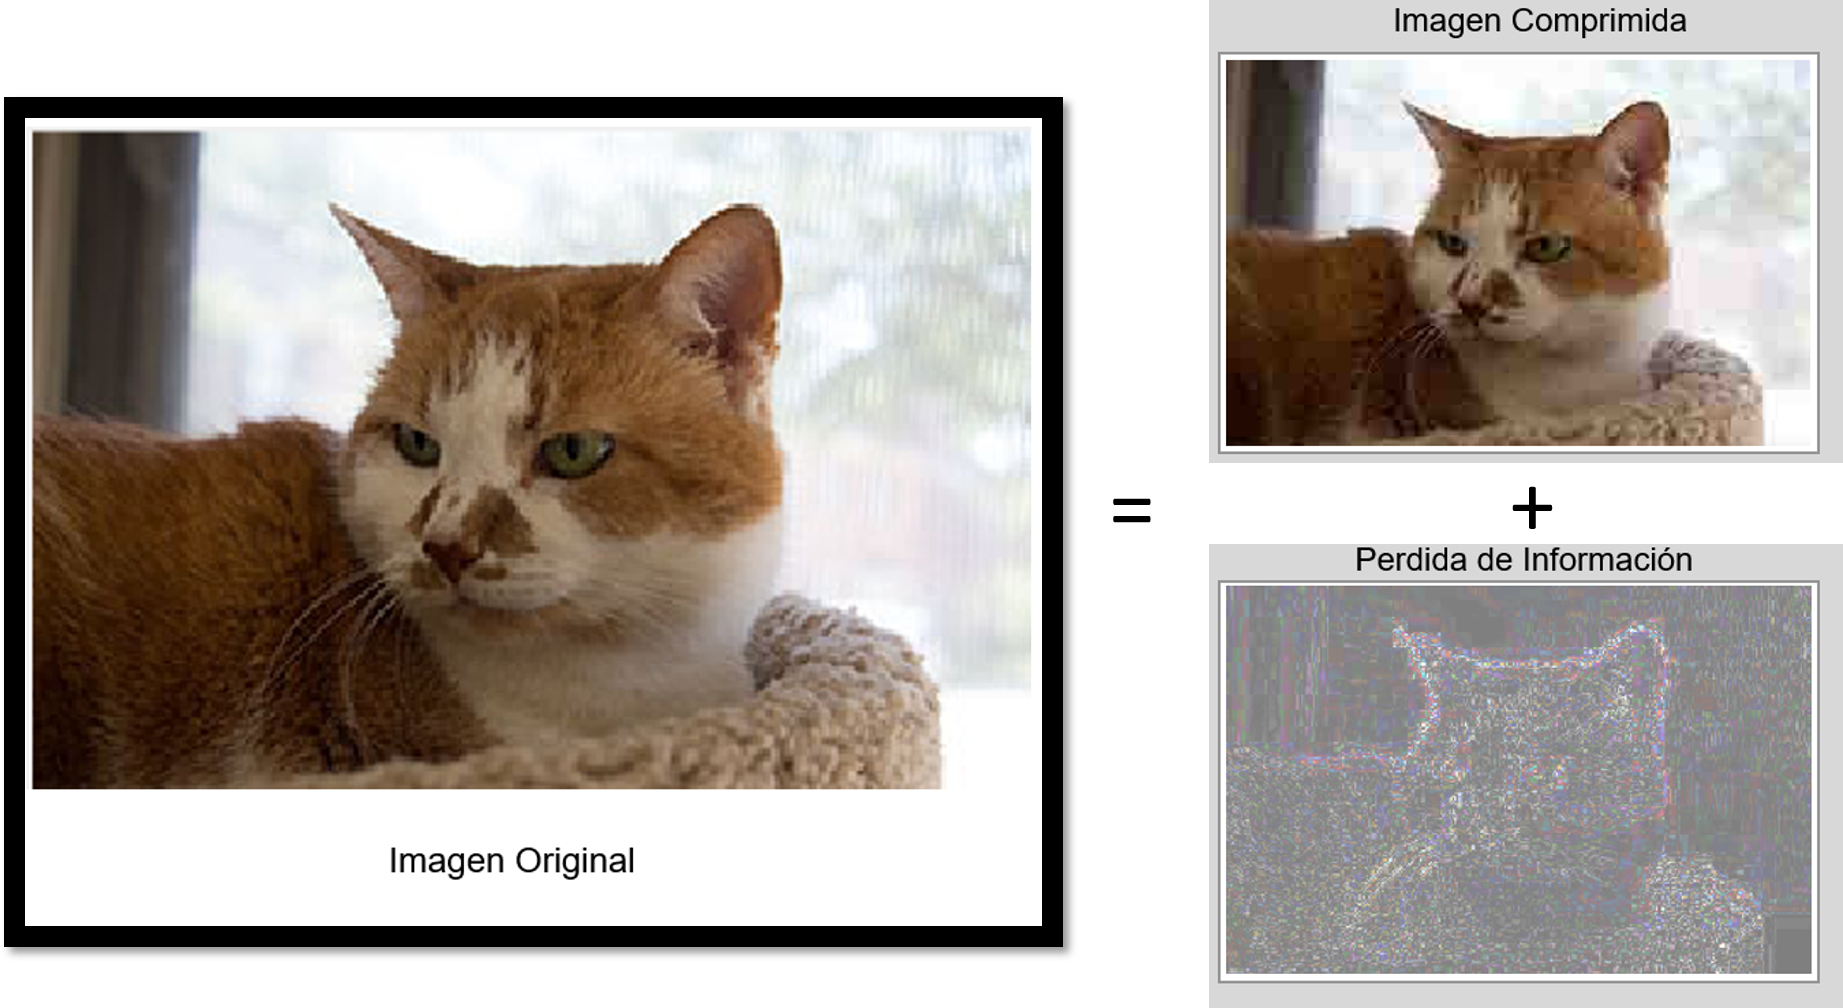
\includegraphics[height=7cm]{imagenes/c2.png}
            \caption{Ejemplo de compresión de datos con perdida (JPG)}
        \end{figure}
    \subsection{Códigos de Huffman}
    David Huffman fue un pionero en su tiempo en el campo de ciencias de la computación, ya que realizó importantes atribuciones en diseño de señales en telecomunicaciones, pero el más popular fue su algoritmo de compresión de datos sin pérdida de información, conocido como codificación de Huffman.
    
    El algoritmo de Huffman crea un árbol binario a partir de las frecuencias de caracteres o símbolos en una cadena. Una vez terminado del árbol se crea una tabla donde cada símbolo le corresponde un código binario único, donde los símbolos con mayor frecuencia tienen un código binario de menor longitud respecto a los códigos de los símbolos de menor frecuencia. Finalmente se construye una nueva cadena sustituyendo los símbolos por su respectivo código logrando con ello una compresión de datos importante para los símbolos con mayor frecuencia.
    \subsection{Algoritmo de Huffman}
        \hyperlink{Anexo}{\large{Vease anexo}}
    \subsection{Histograma de una imagen}
    Un histograma es una representación gráfica de los niveles de exposición que tiene una imagen. Si una imagen es a color, esta tendría 3 histogramas para cada uno de sus canales: rojo, verde y azul. Por el contrario, si solo tiene un canal estamos hablando de una imagen a escala de grises.
    Cada píxel de la imagen tiene el tamaño de un byte, por lo que su valor está en el rango de 0 a 255, entre mayor es el número, mayor exposición tiene el píxel. Por lo tanto, el histograma es una función que mide la frecuencia de todos los píxeles de la imagen y nos indica el nivel de exposición global de la imagen.
    \section{Experimentaci\'on y resultados}
    Se implementó el código de Huffman en Matlab R2020b, ya que nos facilita el manejo de matrices, imágenes e histogramas.
    
    El funcionamiento del código es el siguiente:
    \begin{enumerate}
    \item Cargamos una imagen BMP en escala de grises y se muestra en pantalla.
    \item Calculamos el histograma y se muestra su gráfica.
    \item Preguntamos al usuario cuantos valores desea escoger de la imagen.
    \item Creamos una nueva imagen con la cantidad de valores seleccionados.
    \item Calculamos los códigos de Huffman y se muestran en pantalla.
    \item Se codifica cada fila de la imagen con la tabla de códigos de Huffman.
    \item Mostramos la Imagen Codificada.
    \item Descodificamos la imagen.
    \item Mostramos la imagen Descodificada.
    \item Se imprime el valor de compresión respecto a la imagen original.
    \end{enumerate}
    
    Para nuestro primer caso escogimos una imagen de 16x16 píxeles para poder mostrar paso a paso su ejecución.
    A continuación se muestra la figura junto con sus valores de cada píxel.
    \begin{figure}[H]
            \centering
            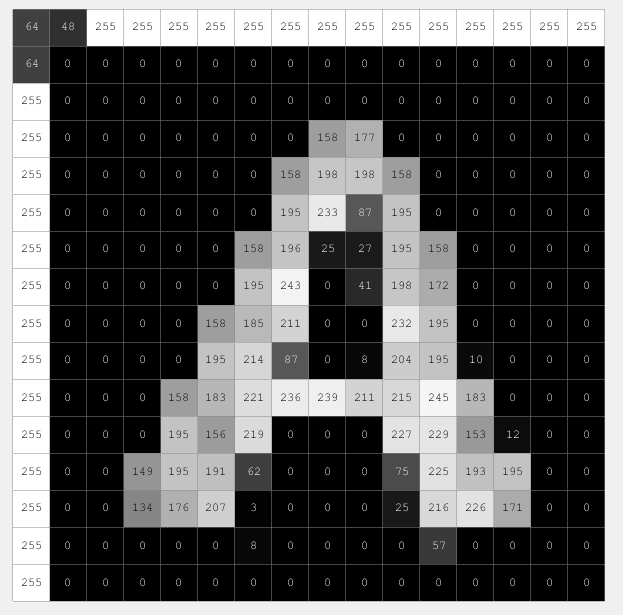
\includegraphics[height=6cm]{imagenes/a1.png}
            \caption{Imagen de 16x16 píxeles}
    \end{figure}
        
    La siguiente figura muestra la imagen original, la imagen con valores reducidos a 8 y la imagen codificada, cada una con su respectivo histograma.
    
    \begin{figure}[H]
            \centering
            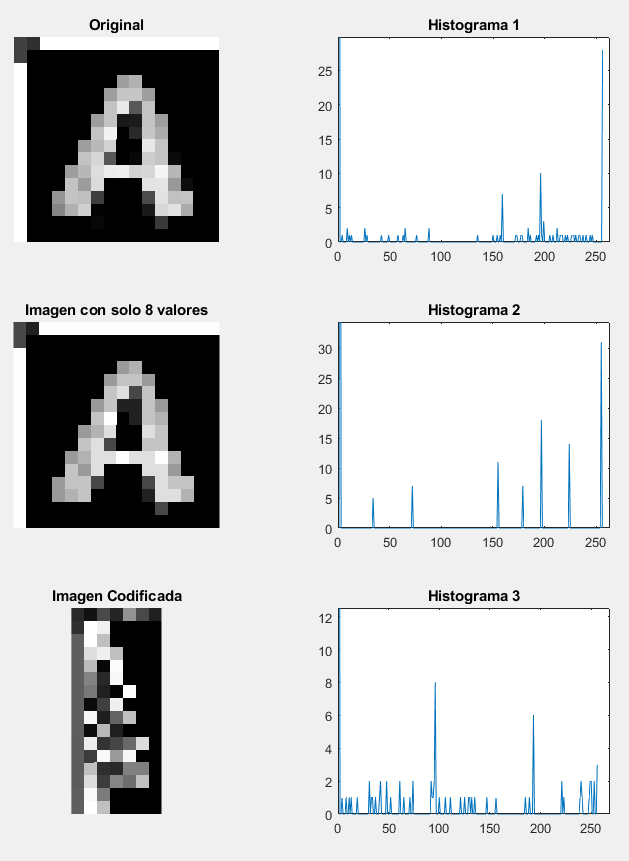
\includegraphics[height=11cm]{imagenes/a2.png}
            \caption{Imágenes e histogramas, ejemplo 1}
        \end{figure}
    
    Como puede observarse en los histogramas, lo que se logra al codificar la figura es que el histograma tiende a tener un comportamiento plano, ya que la entropía aumenta debido a que cada valor aumenta su probabilidad. Otro punto que destaca la imagen codificada es que se aprecia como si se tratara de ruido blanco.\\
    Posteriormente se muestra los códigos de Huffman para cada uno de los 8 valores seleccionados, logrando una compresión al 43.75 por ciento respecto a la imagen original.
    
    \begin{figure}[H]
            \centering
            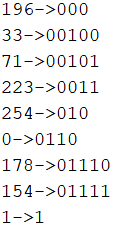
\includegraphics[height=3.5cm]{imagenes/a3.png}
            \caption{Códigos de Huffman, ejemplo 1}
        \end{figure}
    
    El siguiente ejemplo muestra un caballo con diferentes tonos de grises mientras que el fondo de la imagen es color negro.
    
    \begin{figure}[H]
            \centering
            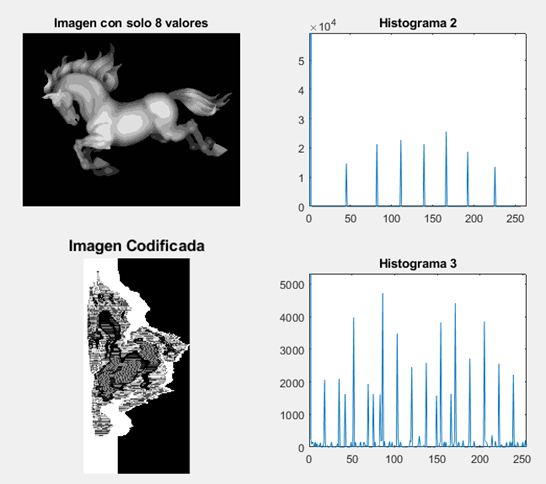
\includegraphics[height=8cm]{imagenes/a4.png}
            \caption{Imágenes e histogramas, ejemplo 2}
        \end{figure}
    \newpage
    
    A continuación se muestran los códigos de Huffman junto con el nivel de compresión respecto a la imagen original.
    
    \begin{figure}[H]
            \centering
            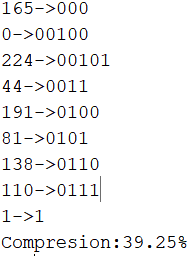
\includegraphics[height=3cm]{imagenes/a7.png}
            \caption{Códigos de Huffman del ejemplo 2}
        \end{figure}
    
    Ahora realizaremos la codificación de Huffman para una imagen BMP donde la mayoría de sus píxeles son de un blanco puro.
    
    \begin{figure}[H]
            \centering
            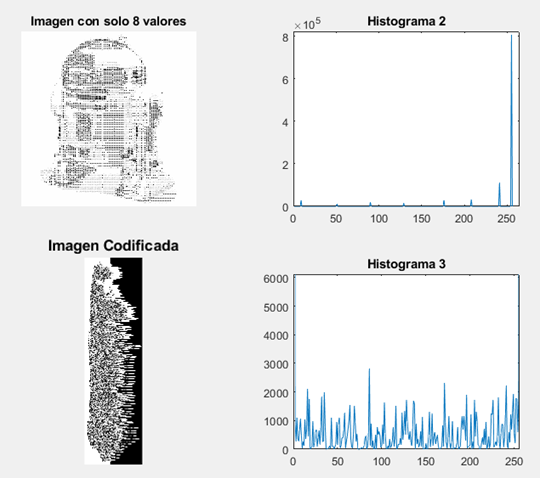
\includegraphics[height=10cm]{imagenes/a5.png}
            \caption{Imágenes e histogramas, ejemplo 3}
        \end{figure}
    
    A continuación se presentan los códigos de Huffman para el ejemplo 3:
    \begin{figure}[H]
            \centering
            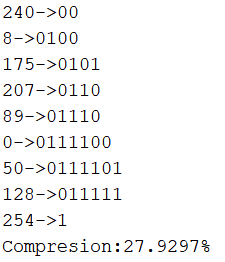
\includegraphics[height=3cm]{imagenes/a6.png}
            \caption{Códigos de Huffman del ejemplo 3}
        \end{figure}
    Como puede observarse en los ejemplos anteriores, la compresión aumenta cuando el histograma tiene un pico muy importante en un valor especifico, como lo puede ser el negro o el blanco, sin embargo, cuando se aumenta el numero de valores seleccionados y el histograma de la imagen original tiene un comportamiento plano, entonces el nivel de compresión disminuye.
    
    En cuanto a la decodificación de las imágenes fue clave mandar como argumentos tanto los códigos de Huffman como el ancho de la imagen  a la función descodificar(), ya que sin ellos no sería posible recuperar la imagen original, por lo que se tiene el comportamiento de un sistema de criptografía si los datos mencionados fueran privados. 
    
    A continuación se mostraran las imágenes decodificadas respecto a las imágenes originales:
    
    \begin{figure}[H]
            \centering
            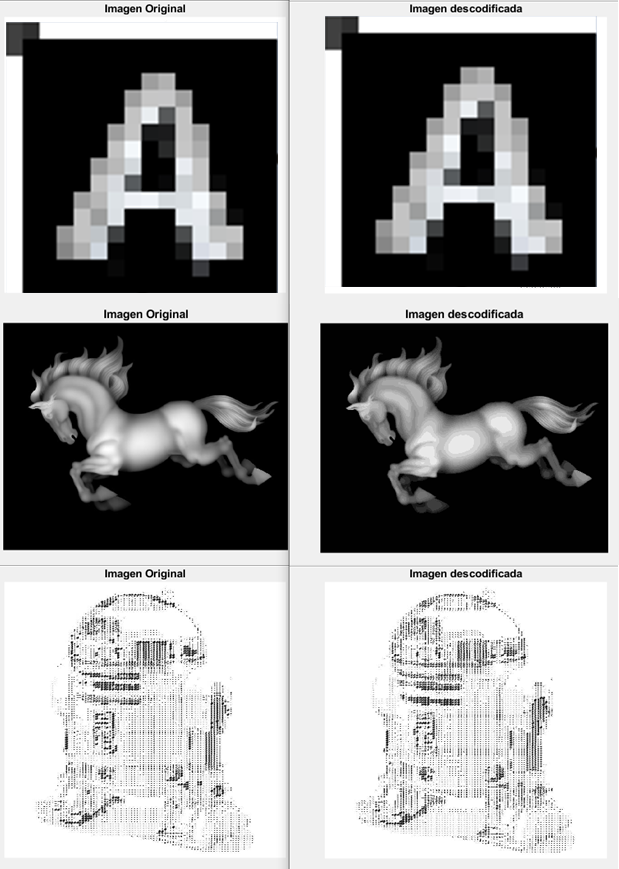
\includegraphics[height=8cm]{imagenes/a8.png}
            \caption{Decodificación de las imágenes de ejemplos 1, 2 y 3}
        \end{figure}
    
    \newpage
    En cuanto a mejoras de este algoritmo podemos mencionar que a la implementación de códigos de Huffman utilizamos el valor 0 como fin de linea, por ello este símbolo está dentro de la codificación de Huffman, y para lograr esto, antes de codificar la imagen nos aseguramos de que todos los píxeles con valor cero fueran sustituidos por unos. De esta manera, la decodificación se logra sin importar los valores que se hayan escogido.
    
    Dado que se ha optado en esta practica por codificar linea a linea, se ha observado que las imágenes codificadas pierden la información visual y no se distinguen correctamente las formas ni el color, por lo que podemos enfocarnos en maximizar la compresión de la imagen sin importar su visualización en estado codificado, es decir, en vez de codificar linea por linea, codificar toda la imagen como si se tratara de una sola linea, ya que con este procedimiento podemos comprimir más la imagen debido a los espacios en negro que cada linea contenía al final de la misma.
    
    \section{Conclusiones}
    
    \textbf{\large Luis Francisco Renteria Cedillo}
    \begin{figure}[H]
        \centering
        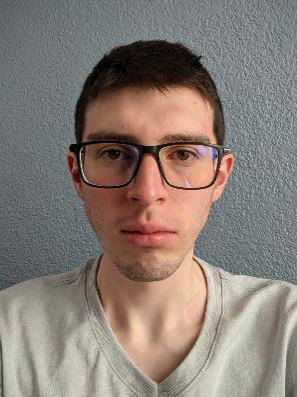
\includegraphics[angle=0, scale=0.5]{imagenes/foto1.png}
    \end{figure}
    
    Se ha observado que la compresión de datos utilizando codificación de Huffman es muy efectiva en cuanto reducción del volumen de información, sin embargo, para imágenes, la imagen codificada pierde la forma, el color y la textura, por lo que no se identifican los elementos presentes en ella. 
    Por otra parte, la compresión JPG aplica la transformada discreta de cosenos a subregiones de la imagen, comúnmente de 8x8 píxeles, logrando deshacerse de las frecuencias más bajas, y al realizar la transformada inversa, no se perciben cambios notables en la imagen, debido a que el cerebro humano reconoce más fácil cambios bruscos de exposición, es decir, las frecuencias altas. Sin embargo, si se tratara de comprimir texto plano, el formato JPG no es factible dado a que se perdería totalmente la información del texto plano, en este caso, la codificación de Huffman es un claro ganador.
    \\\\
    \textbf{\large Denzel Omar Vazquez Perez}
        \begin{figure}[H]
            \centering
            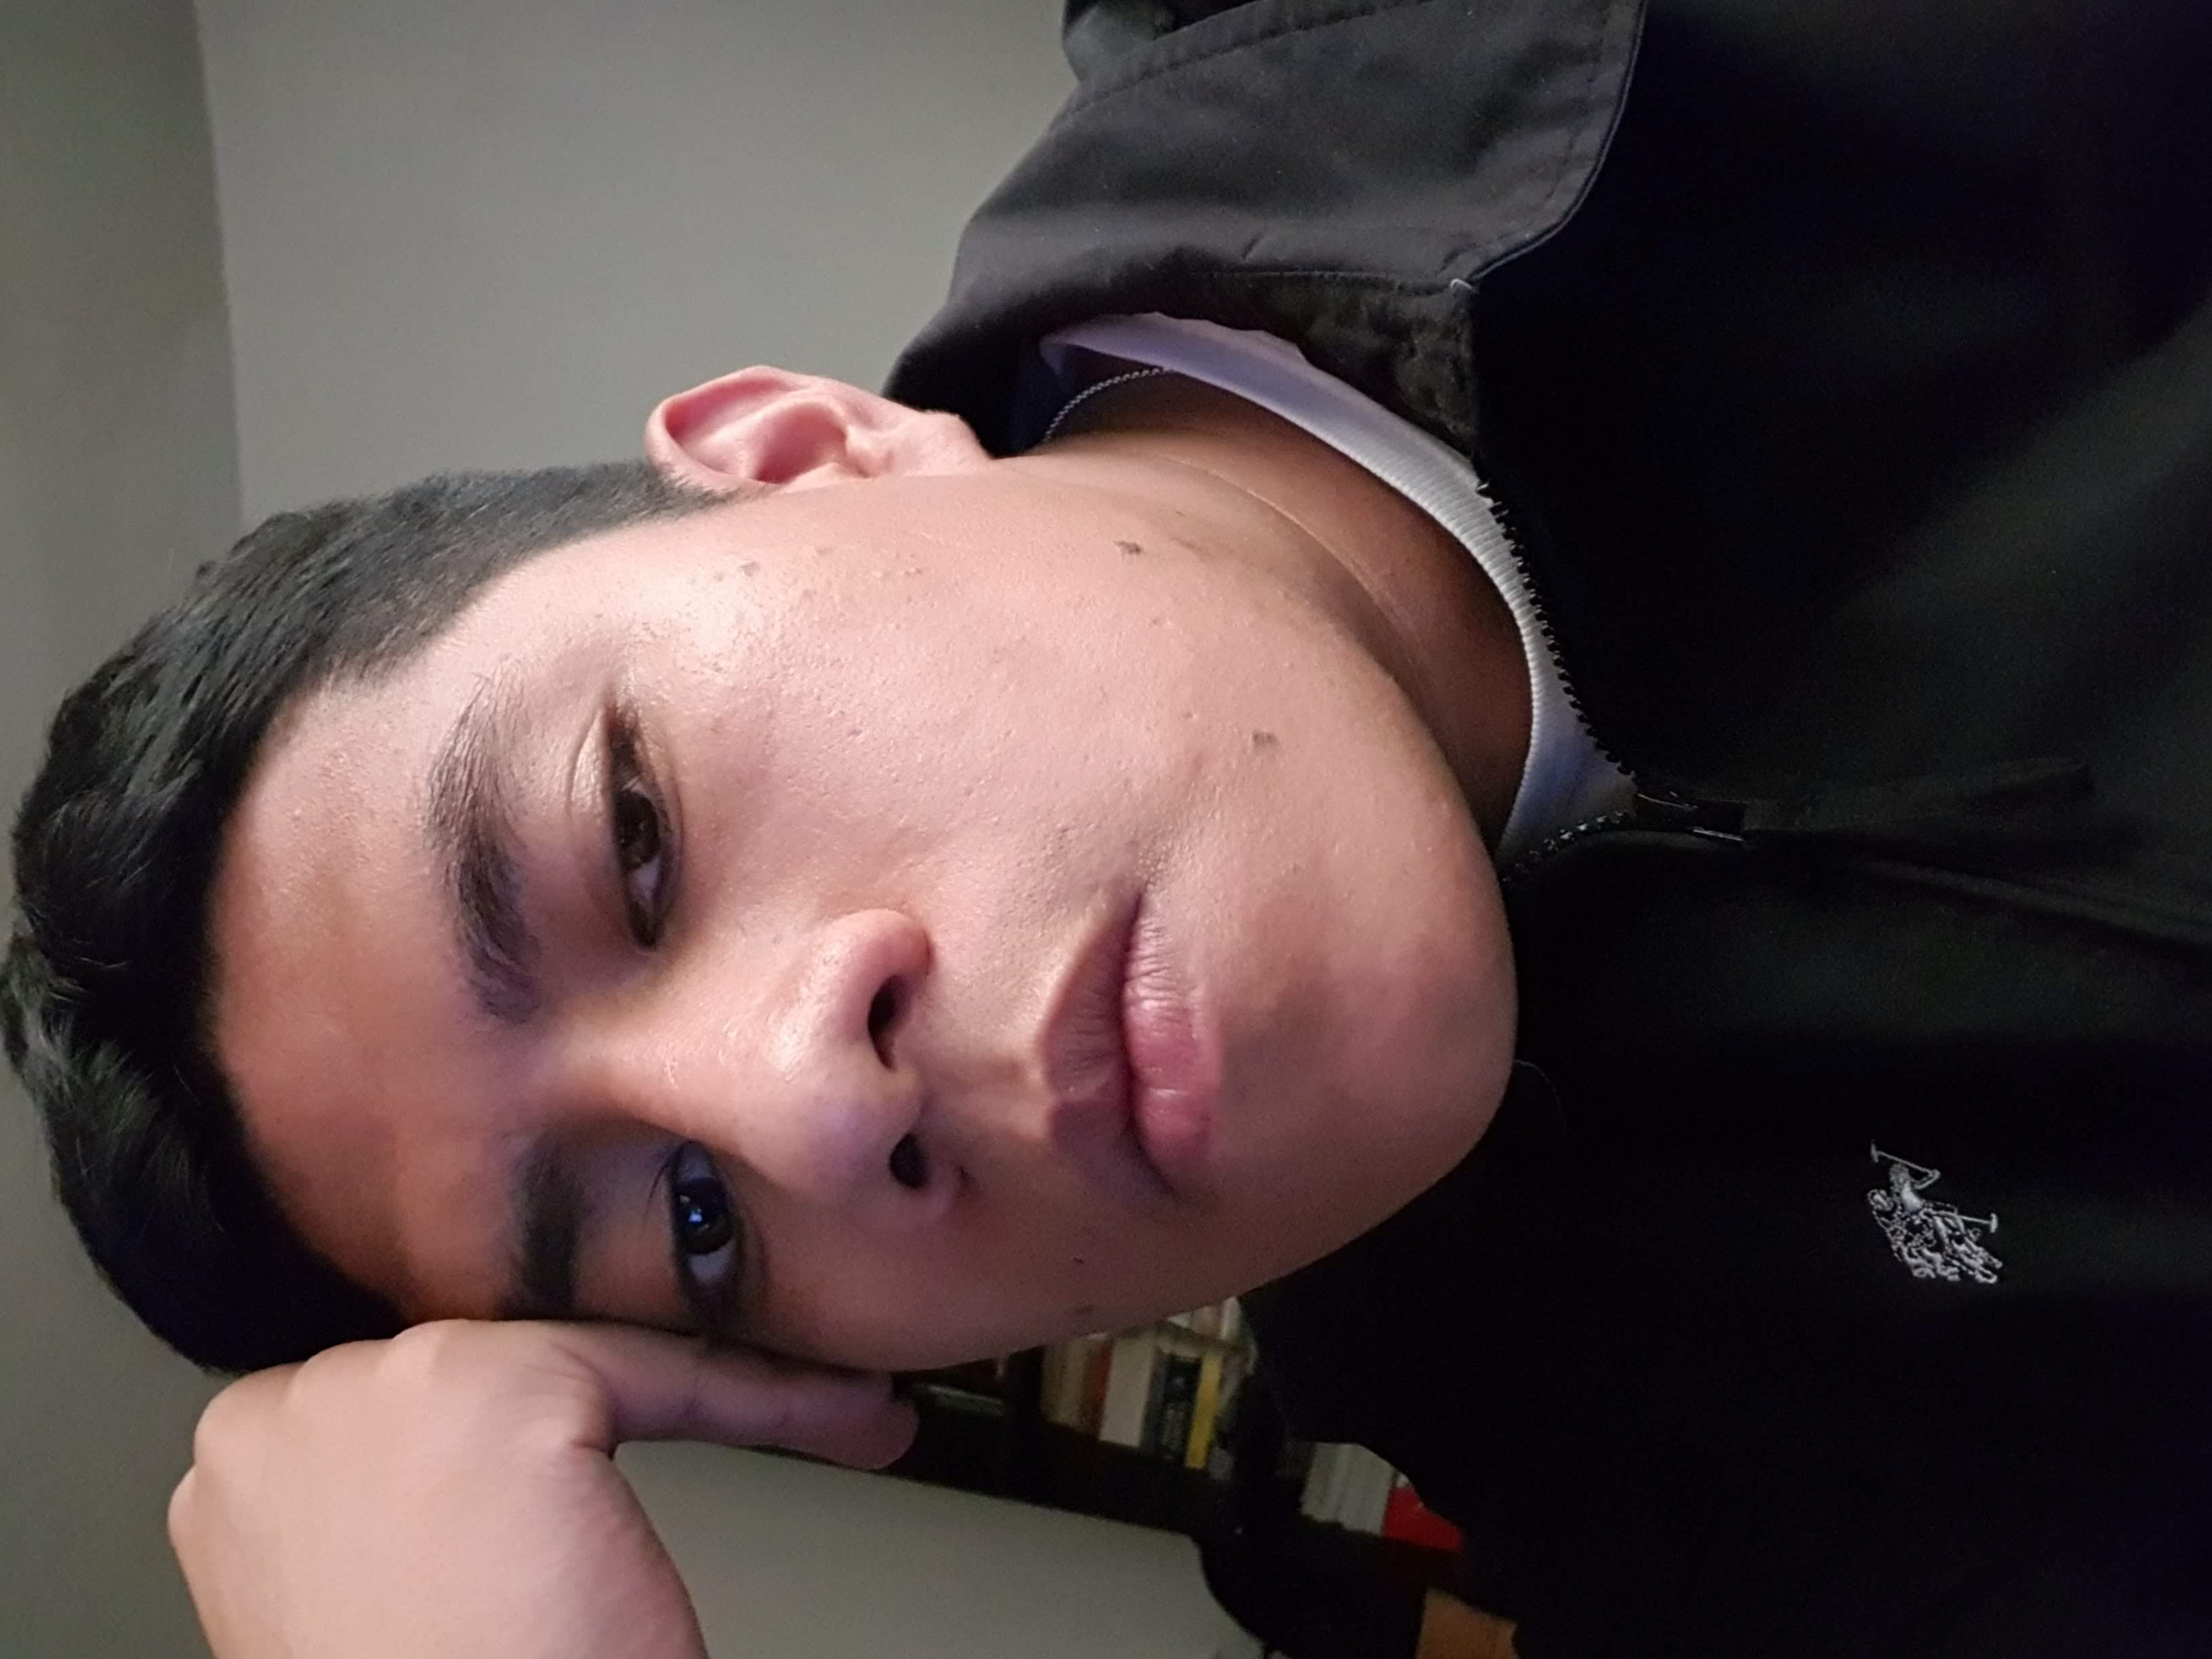
\includegraphics[angle=-90, scale= 0.05]{imagenes/foto2.jpg}
        \end{figure}
    Dada la complejidad del algoritmo de Huffman y al ser un algoritmo de codificaci\'on en prefijo, se asegura que al instante de descodificar la cadena de bits generada por esta no se presentara ninguna ambigüedad, sin embargo su aplicaci\'on en im\'agenes muestra que formas inusuales, como ver pinturas abstractas en una galer\'ia en pleno siglo XXI, y es que a simple vista no se identifica la imagen original en la codificaci\'on, sin embargo se podría mencionar que se muestra un mapa de intensidades de la imagen.
    
    Las mejoras impuestas en permitieron seguir con esa secuencia en prefijo, lo que permiti\'o inmediatamente la descodificaci\'on de lo antes hecho con Huffman.
    
    As\'i resulta interesante cada uno de los resultados presentados en la practica abriendo cada vez mas el panorama a mas aplicaciones relacionadas a los algoritmo voraces vistos en clase, en lo particular nunca hab\'ia trabajado con im\'agenes y se me es emocionante y un nuevo campo con el que seguir trabajando desde hoy en d\'ia.
    
    
    
    \newpage
    \section{Anexo}
    \subsection{Orden de complejidad del algoritmo de mochila fraccionaria}
    Dado el conjunto de {\bf N} art\'iculos cada uno con un {\bf B} beneficio con {\bf w} peso y la capacidad total de la mochila , donde el objetivo es encontrar el valor m\'aximo de fracciones de art\'iculos que pueden caber en la mochila. Por tanto, como se muestra en la Figura 10 se tiene el siguiente algoritmo para cumplir este problema, as\'i se muestra el an\'alisis por bloques de c\'odigo que determina que la complejidad del algoritmo es $T(n)\in\mathcal{O}(n\log(n))$ ante el peor caso de mochila fraccionaria.
    \begin{figure}[H]
        \centering
        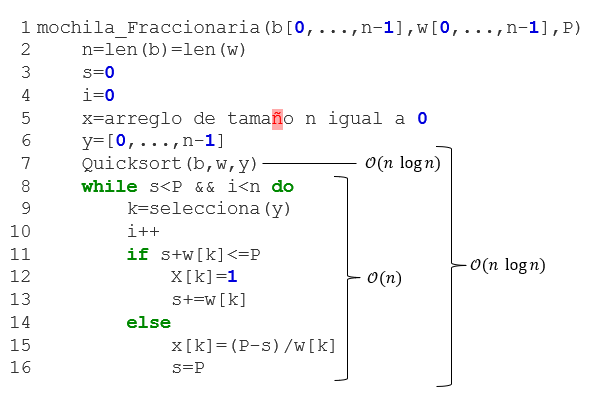
\includegraphics[height=7cm]{imagenes/complejidad_mochila.png}
        \caption{Algoritmo de mochila fraccionaria}
    \end{figure}
    \subsection{Contraejemplo del algoritmo de mochila fraccionaria}
        {\bf Sol.}\\
        Si se cuenta con una mochila de peso maximo P=8 y 4 objetos enteros no fraccionables, donde cada articulo tiene un peso $w_i$ y un beneficio $b_i$, se tiene los siguientes pesos [4,3,5,2] y beneficios [10,40,30,20].\\\\
        Por tanto el algoritmo voraz selecciona $W_{1,3}$ ya que son los objetos que entran dentro de la mochila para obtener
        $$M_w=3+2=5~y~M_b=40+20=60$$
        A simple vista se observa que la el peso obtenido no alcanza el m\'aximo que puede soportar la mochila, ya que exceder\'a esta misma al agregar otro articulo. Sin embargo existe una soluci\'on \'optima escogiendo $w_{1,2}$ 
        $$M_w=3+5=8~y~M_b=40+30=70$$
        Por tanto se demuestra que el algoritmo voraz de mochila fraccionaria al elegir objetos enteros no genera soluciones \'optimas.
            
    \subsection{¿Cu\'al sería la mejor funci\'on de selección voraz en el caso en el que todos los objetos tuvieran el mismo valor?}
        Para obtener una soluci\'on \'optima se tendr\'an que elegir aquellos art\'iculos con el mayor beneficio por el peso que puede soportar la mochila.
    
    \subsection{¿Cu\'al ser\'ia la mejor funci\'on de selecci\'on voraz en el caso en el que todos los objetos tuvieran el mismo peso?}
        Para obtener una soluci\'on \'optima se tendr\'an que elegir aquellos art\'iculos con el mayor peso por el beneficio que adquiere la mochila.
        
    \subsection{Construir la codificación de Huffman para la cadena: ciencias de la tierra}
    {\bf Sol.}
    Dada la cadena {\it "ciencias de la tierra"} se contruye la tabla de frecuencias de los caracteres contenidos en este, vease Tabla 1.
    \begin{longtable}{|c|c|c|c|c|c|c|c|c|c|c|c|}
        \caption{Tabla de frecuencias de los caracteres de la cadena {\it ciencias de la tierra}}\\
        \hline
             &{}&{a}&{c}&{d}&{e}&{i}&{l}&{n}&{r}&{s}&{t}\\
        \hline
            {Frecuencia}&{3}&{3}&{2}&{1}&{3}&{3}&{1}&{1}&{2}&{1}&{1}\\
        \hline
    \end{longtable}
    As\'i dados los resultados de la Tabla 1, se procede a ordenar los caracteres de mayor a menor frecuencia, v\'ease Tabla 2.
    \begin{longtable}{|c|c|c|c|c|c|c|c|c|c|c|c|}
        \caption{Tabla de frecuencias ordenada}\\
        \hline
             &{}&{a}&{e}&{i}&{c}&{r}&{d}&{l}&{n}&{s}&{t}\\
        \hline
            {Frecuencia}&{3}&{3}&{3}&{3}&{2}&{2}&{1}&{1}&{1}&{1}&{1}\\
        \hline
    \end{longtable}
    Por tanto haciendo usos de la Tabla 2 , se construye el \'arbol de frecuencias
    \begin{longtable}{|c|c|c|c|c|c|c|c|c|c|c|}
        \hline
            {d}&{l}&{n}&{s}&{t}&{c}&{r}&{ }&{a}&{e}&{i}\\
        \hline
            {1}&{1}&{1}&{1}&{1}&{2}&{2}&{3}&{3}&{3}&{3}\\
        \hline
    \end{longtable}
    \begin{center}
        \begin{tikzpicture}
            \node{2} [sibling distance=2cm]
                child {node {d,1} [sibling distance=1.5cm]}
                child{node{l,1}};
        \end{tikzpicture}
    \end{center}
    \begin{longtable}{|c|c|c|c|c|c|c|c|c|c|}
        \hline
            {n}&{s}&{t}&{d,l}&{c}&{r}&{ }&{a}&{e}&{i}\\
        \hline
            {1}&{1}&{1}&{2}&{2}&{2}&{3}&{3}&{3}&{3}\\
        \hline
    \end{longtable}
    \begin{center}
        \begin{tikzpicture}
            \node{2} [sibling distance=2cm]
                child {node {n,1} [sibling distance=1.5cm]}
                child{node{s,1}};
        \end{tikzpicture}
    \end{center}
    \begin{longtable}{|c|c|c|c|c|c|c|c|c|}
        \hline
            {t}&{n,s}&{d,l}&{c}&{r}&{ }&{a}&{e}&{i}\\
        \hline
            {1}&{2}&{2}&{2}&{2}&{3}&{3}&{3}&{3}\\
        \hline
    \end{longtable}
    \begin{center}
        \begin{tikzpicture}
            \node {3} [sibling distance=2cm]
            child {node {t,1} [sibling distance=1.5cm]}
            child{node{2}
                    child{node{n,1}}
                    child{node{s,1}}};
        \end{tikzpicture}
    \end{center}
    \begin{longtable}{|c|c|c|c|c|c|c|c|}
        \hline
            {d,l}&{c}&{r}&{t,n,s}&{ }&{a}&{e}&{i}\\
        \hline
            {2}&{2}&{2}&{3}&{3}&{3}&{3}&{3}\\
        \hline
    \end{longtable}
    \begin{center}
        \begin{tikzpicture}
            \node {4} [sibling distance=2cm]
            child{node{2}[sibling distance=1.5cm]
                    child{node{d,1}}
                    child{node{l,1}}}
            child {node {c,2}};
        \end{tikzpicture}
    \end{center}
    \begin{longtable}{|c|c|c|c|c|c|c|}
        \hline
            {r}&{t,n,s}&{ }&{a}&{e}&{i}&{d,l,c}\\
        \hline
            {2}&{3}&{3}&{3}&{3}&{3}&{4}\\
        \hline
    \end{longtable}
    \begin{center}
        \begin{tikzpicture}
            \node {5} [sibling distance=2cm]
                child {node {r,2} [sibling distance=1.5cm]}
                child {node{3}
                    child{node{t,1}}
                    child{node{2}
                        child{node{n,1}}
                        child{node{s,1}}
                    }
                };
        \end{tikzpicture}
    \end{center}
    \begin{longtable}{|c|c|c|c|c|c|}
        \hline
            { }&{a}&{e}&{i}&{d,l,c}&{r,t,n,s}\\
        \hline
            {3}&{3}&{3}&{3}&{4}&{5}\\
        \hline
    \end{longtable}
    \begin{center}
        \begin{tikzpicture}
            \node{6} [sibling distance=2cm]
                child {node { ,3} [sibling distance=1.5cm]}
                child{node{a,3}};
        \end{tikzpicture}
    \end{center}
    \begin{longtable}{|c|c|c|c|c|c|}
        \hline
            {e}&{i}&{d,l,c}&{r,t,n,s}&{ ,a}\\
        \hline
            {3}&{3}&{4}&{5}&{6}\\
        \hline
    \end{longtable}
    \begin{center}
        \begin{tikzpicture}
            \node{6} [sibling distance=2cm]
                child {node {e,3} [sibling distance=1.5cm]}
                child{node{i,3}};
        \end{tikzpicture}
    \end{center}
    \begin{longtable}{|c|c|c|c|c|}
        \hline
            {d,l,c}&{r,t,n,s}&{e,i}&{ ,a}\\
        \hline
            {4}&{5}&{6}&{6}\\
        \hline
    \end{longtable}
    \begin{center}
        \begin{tikzpicture}
            \node {9} [sibling distance=5cm]
            child {node {4} [sibling distance=1.5cm]
                child{node{2}
                    child{node{d,1}}
                    child{node{l,1}}
                }
                child{node{c,2}}
            }
            child{node{5} [sibling distance=1.5cm]
                child{node{r,2}}
                child{node{3}
                    child{node{t,1}}
                    child{node{2}
                        child{node{n,1}}
                        child{node{s,1}}
                    }
                }
            };
        \end{tikzpicture}
    \end{center}
    \begin{longtable}{|c|c|c|}
        \hline
            {e,i}&{ ,a}&{d,l,c,r,t,n,s}\\
        \hline
            {6}&{6}&{9}\\
        \hline
    \end{longtable}
    \begin{center}
        \begin{tikzpicture}
            \node {12} [sibling distance=3cm]
            child{node{6}[sibling distance=2cm]
                    child{node{e,3}}
                    child{node{i,3}}
                }
            child{node {6}[sibling distance=2cm]
                child {node { ,3}}
                child{node{a,3}}
            };
        \end{tikzpicture}
    \end{center}
    \begin{longtable}{|c|c|}
        \hline
            {d,l,c,r,t,n,s}&{e,i, ,a}\\
        \hline
            {9}&{12}\\
        \hline
    \end{longtable}
    \begin{center}
        \begin{tikzpicture}
            \node {21} [sibling distance=6cm]
            child{node {9} [sibling distance=3cm]
                child {node {4} [sibling distance=1.5cm]
                    child{node{2}
                        child{node{d,1}}
                        child{node{l,1}}
                    }
                    child{node{c,2}}
                }
                child{node{5} [sibling distance=1.5cm]
                    child{node{r,2}}
                    child{node{3}
                        child{node{t,1}}
                        child{node{2}
                            child{node{n,1}}
                            child{node{s,1}}
                        }
                    }
                } 
            }
            child{node {12} [sibling distance=2cm]
                child{node{6}[sibling distance=1.5cm]
                        child{node{e,3}}
                        child{node{i,3}}
                    }
                child{node {6}[sibling distance=1.5cm]
                    child {node { ,3}}
                    child{node{a,3}}
                }
            };
        \end{tikzpicture}
    \end{center}
    Se observa que cada nodo ra\'iz puede solo tener un nodo hijo izquierdo como derecho, por lo que colocando un 0 y 1 respectivamente, se obtiene la siguiente codificaci\'on de Huffman, v\'ease Tabla 13.
    \begin{longtable}{|c|c|}
        \caption{Codificaci\'on Huffman}\\
        \hline
            {car\'acter}&{c\'odigo}\\
        \hline
            {c}&{001}\\
        \hline
            {r}&{010}\\
        \hline
            {e}&{100}\\
        \hline
            {i}&{101}\\
        \hline
            { }&{110}\\
        \hline
            {a}&{111}\\
        \hline
            {d}&{0000}\\
        \hline
            {l}&{0001}\\
        \hline
            {t}&{0110}\\
        \hline
            {n}&{01110}\\
        \hline
            {s}&{01111}\\
        \hline
    \end{longtable}
    
    Finalmente la codificaci\'on de Huffman de la cadena {\it "ciencias de la tierra"} a partir de la Tabla 13 es:\\
    \begin{center}
        {\Large ciencias de la tierra }\\
        0011011000111000110111101111{\bf 110}0000100{\bf 110}0001111{\bf 110}0110101100010010111  
    \end{center}
    \subsection{Orden de complejidad del algoritmo de Huffman}
        \hypertarget{Anexo}{El algoritmo de Huffman} hace la compresi\'on de datos sin perdidas asignando c\'odigos en prefijo de longitud variable a los caracteres que reciba este, estos se generan a partir de frecuencias de los caracteres \'unicos de la cadena. Donde el car\'acter m\'as frecuente obtiene el c\'odigo m\'as preque\~no y el car\'acter menos frecuente obtiene el c\'odigo m\'as grande, de este modo se asegura que no exista la ambigüedad al decodificar la cadena de bits generada. As\'i se muestra en la Figura 11 el an\'alisis por bloques de c\'odigo determina que la complejidad del algoritmo es $T(n)\in\mathcal{O}(n\log(n))$ ante el peor caso de Huffman.
        \begin{figure}[H]
        \centering
        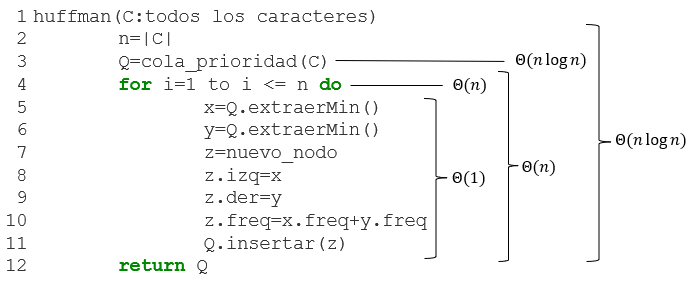
\includegraphics[height=5cm]{imagenes/complejidad_huffman.png}
        \caption{Algoritmo de Huffman}
    \end{figure}
    \subsection{Orden de complejidad del algoritmo de Kruskal}
        El algoritmo de Kruskal representa un \'arbol de expansi\'on m\'nimo que hace usos de un grafo encontrando un subconjunto de aristas de este que formen un \'arbol con todos los nodos obteniendo la suma de costos mínimos entre todos los arboles que puede generar para obtener un \'optiomo local, que pueda ser el global. As\'i se muestra en la Figura 12 el an\'alisis por bloques de c\'odigo que determina que la complejidad del algoritmo es $T(n)\in\mathcal{O}(n\log(n))$ ante el peor caso de este.   
        \begin{figure}[H]
        \centering
        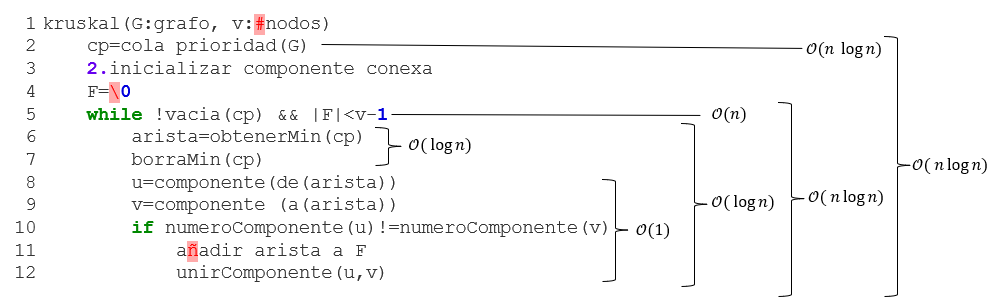
\includegraphics[height=4cm]{imagenes/complejidad_kruskal.png}
        \caption{Algoritmo de Kruskal}
    \end{figure}
    \newpage
    \subsection{Algoritmo Prim} 
    El algoritmo de Prim incrementa el \'arbol de expasi\'on m\'inimo comenzando por un v\'ertice inicial al que sucesivamente se le a\~aden v\'ertices cuya distancia a los padres sea m\'inima, as\'i cada arista que aparece es por la coincidencia de vertices en el \'arbol. El presente pseudo-c\'odigo determina que la complejidad del algoritmo es $T(n)\in\mathcal{O}(n\log(n))$ ante el peor caso de este.
    \begin{algorithm}[H]
        \caption{ Prim(G:grafo)}
        \begin{algorithmic}[1]
        \For{0 to $|V|-1$} 
            \State D[u]=INFINITO
            \State Parent[u]=NULL
            \State Insert(Q,u)
        \EndFor
		\State D[u]=0
		\While {!isempty(Q)}
		    \State u=min(Q)
		    \For{$each \in Adj[u]$}
		        \If{$(v\in Q)~\&\&~(D[v])>w(u,v)$}
		            \State Parent[v]=u
		            \State D[v]=w(u,v)
		            \State update(Q,v,D[v])
		        \EndIf
		    \EndFor
		\EndWhile
        \end{algorithmic}
    \end{algorithm}
        
    \subsection{Orden de complejidad del algoritmo de Dijkstra}
        El algoritmo de Dijkstra, es una util herramienta para encontrar el camino mas corto o con menor costo entre todos lo nodos del grafo, a partir de un {\it "nodo inicial"}, a diferencia del \'arbol de expasi\'on m\'inimo este no hace uso de todos lo v\'ertices del grafo. As\'i se muestra en la Figura 13 el an\'alisis por bloques de c\'odigo que determina que la complejidad del algoritmo es $T(n)\in\mathcal{O}(n^2))$ ante el peor caso del algoritmo.
        \begin{figure}[H]
        \centering
        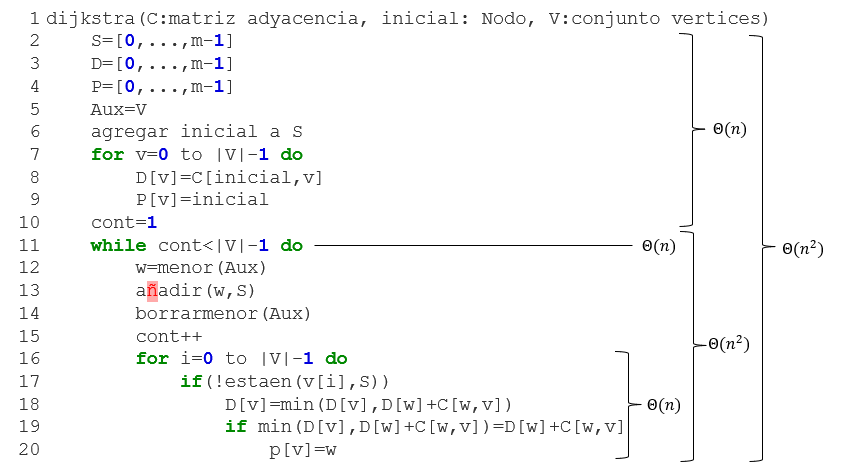
\includegraphics[height=6cm]{imagenes/complejidad_dijkstra.png}
        \caption{Algoritmo de Dijkstra}
        
    \end{figure}
    \section{Bibliograf\'ia}
    Brassard, G. (1997). \textit {Fundamentos de Algoritmia}. España: Ed. Prentice Hall.\\[0.4cm]
    Cormen, E. A. (2022). \textit{Introduction To Algorithms}, 3Rd Ed. Phi.\\[0.4cm]
    S\'anchez, P. J. I. (2006). \textit{Análisis y diseño de algoritmos: un enfoque teórico y práctico}. Servicio de Publicaciones y Divulgación Científica de la UMA.\\[0.4cm]
    Nipun Ramakrishnan, Reducible (Julio 2021), \textit{Huffman Codes: An Information Theory Perspective}, Youtube, https://www.youtube.com/watch?v=B3y0RsVCyrw
\end{document}